\chapter{Algorithms and running time analysis} 
\label{cha:runn-time-analys}



An \emph{algorithm} executes a set of \emph{instructions}
used in common programming languages like  arithmetic
operations, comparisons or read/write instructions. The sequence of these instructions is controlled by \emph{loops and conditionals} like {\tt if, while, for} etc. 

Each of these instructions requires \emph{time}. The \emph{running time} of an algorithm is the \emph{number of instructions} that the algorithm performs. This number depends on the \emph{input} of the algorithm. 


\begin{example}
\label{ex-a-1}
  Consider the following algorithm to compute the product of two $n × n$ matrices $A,B ∈ ℚ^{n ×n}$: 
    \begin{tabbing}            
    {\bf for} \= $i=1,\dots,n$ \\ 
              \> {\bf for} \= $j=1,\dots,n$ \\
              \> \> $c_{ij} := 0$ \\
              \> \> {\bf for} \= $k=1,\dots,n$ \\
              \> \> \> $c_{ij} := c_{ij} + a_{ik} ⋅ a_{kj}$
            \end{tabbing} 
%
 The number of additions that are carried out is $n^2 ⋅ (n-1)$ and the number of multiplications is $n^3$.
 The number of store-instructions is $n^2 ⋅(n+1)$. The number of read-instructions is of similar magnitude. 
\end{example}


The above example shows that an \emph{exact counting} is sometimes
tedious. Looking at the algorithm however, you quickly agree that
there exists \emph{some constant} $c \in \R_{>0}$ such that the
algorithm performs at most $c ⋅ n^3$ instructions. 

In the analysis of algorithms, one does usually not care so much about the constant $c$ above in the beginning. There are sub-fields of algorithms where this constant however matters. Especially for algorithms on large data sets, where access to external data is costly. However, this is another story that does not concern us here. When we analyze algorithms, we are interested in the \emph{asymptotic running time}. 

\begin{definition}[$O$-notation]  

 Let $T,f: \setN \to \setR_{\geq0}$ be functions. We say 
  \begin{itemize}
  \item \emph{$T(n) = O(f(n))$}, if there exist positive  constants
    $n_o\in \setN$ and  $c\in\setR_{>0}$ 
    with $$T(n) \leq c \cdot f(n) \text{ for all }n\geq n_0.$$  
  \item \emph{$T(n) = \Omega(f(n))$}, if there exist constants   $n_o\in \setN$
    and  $c\in\setR_{>0}$ 
    with $$T(n) \geq c \cdot f(n)\text{ for all } n\geq n_0.$$
  \item \emph{$T(n) = \Theta(f(n))$}  if $$T(n)=O(f(n))\text{ and }
     T(n) = \Omega(f(n)).$$
  \end{itemize}
\end{definition}


\begin{example}
  The function $T(n)=2n^2 + 3n +1$ is in $O(n^2)$, since for all
  $n\geq1$ one has $2n^2 + 3n + 1 \leq 6n^2$. Here $n_0 = 1$ and $c =
  6$.  Similarly $T(n) = \Omega(n^2)$, since for each $n\geq1$ one has $2n^2 + 3n
  +1\geq n^2$. Thus $T(n)$ is in $\Theta(n^2)$. 
\end{example}

We measure the running time of algorithms in terms of the \emph{length
  of the input}.  The matrices $A$ and $B $ that are the input of the matrix-multiplication
algorithm of Example~\ref{ex-a-1} consist of $n^2$ 
numbers each. The algorithm runs in time $O(n^3 = (n^2)^{3/2})$. 


What does it mean for an algorithm to be efficient? For us, this will
mean that it runs in \emph{polynomial time}. As a first definition of
polynomial time algorithm, we say that an algorithm runs in
\emph{polynomial time}, if there exists a constant $k$ such that the
algorithm runs in time $O(n^k)$, where $n$ is the length of the input
of the algorithm.

However, we recall the \emph{binary} representation of natural numbers $n ∈ ℕ$. A sequence of \emph{bits} $a_0,\dots,a_{k-1}$ with $a_j ∈ \{0,1\}$ for $0 ≤j≤k-1$ represents the number 
\begin{displaymath}
  ∑_{j=0}^{k-1} a_j ⋅ 2^j. 
\end{displaymath}  
Conversely, each positive natural number $n≥1$ has the binary representation that is found recursively by the following process. 
If $n=1$, then its representation is $a_0 = 1$. 
If $n>1$ and  is even, then the sequence representing $n$ is 
\begin{displaymath}
  0,b_0,\dots,b_{k-1},
\end{displaymath}
where $b_0,\dots,b_{k-1}$ is the representation of $n/2$. If $n>1$ and n is odd, then the sequence representing $n$ is 
\begin{displaymath}
  1,b_0,\dots,b_{k-1},
\end{displaymath}
where $b_0,\dots,b_{k-1}$ is the representation of $⌊n/2⌋$. This creates a representation with leading bit one, i.e. $a_{k-1}=1$. 
By deleting \emph{leading zeros}, i.e., ensuring $a_{k-1}=1$, the representation of a natural positive number is unique, (see exercise~\ref{cha:runn-time-analys}.\ref{alg:ex2}). 



\begin{example}
  This example will make us revise the our first definition of a polynomial-time algorithm. 
The input of this algorithm is a list of characters. Let us say that the list has $n$ elements. 
 
 \label{ex-a-3}
  \begin{tabbing}
    Input: A list $L$ or characters \\
    $s :=2$ \\
    {\bf for} \= $c ∈ L$:\\
              \> $s:= s ⋅ s$ \\
    {\bf return} $s$         
  \end{tabbing}
  Then clearly, the algorithm carries out a polynomial, even linear,
  number of operations in the input, if we consider an arithmetic
  operation also as a basic operation that can be carried out in
  constant time. However, the algorithm squares $2$
  repeatedly, $n$
  times to be precise. Thus, at the end, the variable $s$
  holds the number $2^{2^n}$.
  The number of \emph{bits} in the binary representation  that the return value
  is $2^n$
  which is \emph{exponential} in the input length. 
\end{example}

\begin{definition}
  \label{def:2}
  The \emph{size} of an integer $x$
  is $\size(x) = \lceil\log( |x| +1)\rceil$
  and for $x \in \setQ$,
  $\size(x) = \size(p)+\size(q)$,
  where $x = p/q$ with $p,q \in \setZ$, $q\geq1$ and $\gcd(p,q)=1$.   
\end{definition}
Here $\gcd(p,q)$ denotes the \emph{greatest common divisor} of $p$ and $q$ which we define precisely below. 
Thus the size of a number is asymptotically equal to the number of
bits that are needed to store the number.  We now provide the
definition of what a polynomial-time algorithm is.
\begin{definition}
  \label{def:1}
  An algorithm is \emph{polynomial time}, if there exists a
  constant $k$
  such that the algorithm performs $O(n^k)$
  operations on rational numbers whose size is bounded by
  $O(n^k)$.
  Here $n$
  is the number of bits that encode the input of the algorithm. We say that the algorithm runs in time $O(n^k)$. 
\end{definition}

We now use this definition to analyze the famous \emph{Euclidean} algorithm that computes the \emph{greatest common divisor} of two integers. 

 For $a,b \in \setZ$, $b \neq0$ we say $b$ \emph{divides} $a$ if there
    exists an $x \in \setZ$ such that $a = b \cdot  x$. We 
    write    $b\mid a$.  
   For $a,b,c \in \setZ$, if $c\mid a$ and $c\mid b$, then $c$ is a
    \emph{common divisor} of $a$ and $b$. 
    If at least one of the two integers $a$ and $b$ is non-zero,
    then there exists a \emph{greatest common divisor} of $a$ and
    $b$. It is denoted by \emph{$\gcd(a,b)$}. 
    

    How do we compute the greatest common divisor efficiently? The
    following is called \emph{division with remainder}.  For
    $a,b \in \setZ$
    with $b >0$ there exist unique integers $q,r \in \setZ$ with
    \begin{displaymath}
      a = q\cdot b + r, \text{ and }  0\leq r <b. 
    \end{displaymath}
    Now clearly, 
    for $a,b \in \setZ$ with $b >0$ and $q,r \in \setZ$ as above one has
    $\gcd(a,b) = \gcd(b,r)$.  
  This gives rise to the famous \emph{Euclidean algorithm}. 
  \begin{algorithm}[Euclidean algorithm]
    \label{alg:1}
    \begin{tabbing}
      Input: Integers $a ≥ b ≥0$ not both equal to zero \\
      Output: The greatest common divisor $\gcd(a,b)$\\
      {\bf if}  $(b=0)$ {\bf return} $a$ \\
      {\bf else} \= \\
      \> Compute $q,r ∈ ℕ$ with \=  $b > r ≥ 0$ and $a = q⋅b +r$ \\
      \> \> (division with remainder)\\
      \> {\bf return} $\gcd(b,r)$ 
    \end{tabbing}
  \end{algorithm}  
%
  \begin{theorem}
    The Euclidean algorithm runs in time $O(n)$. 
  \end{theorem}
  \begin{proof}
    Suppose that $a$ and $b$ have at most $n$ bits each.  Clearly, the
    numbers in the course of the algorithm have at most $n$
    bits. Furthermore, if $a \geq b$, then $r \leq a/2$, where $r$ is
    the remainder of the division of $a$ by $b$. Thus each second
    iteration, the first parameter of the input has one bit less. Thus
    the number of operations is bounded by $O(n)$.
  \end{proof}
  
\begin{example}
\label{exe:det}
The \emph{determinant} of a matrix $A ∈ ℝ^{n ×n}$ can be computed by the recursive formula 
\begin{displaymath}
  \det(A) = ∑_{i=1}^n (-1)^{1+j}a_{1j} \det(A_{1j}),
\end{displaymath}
where $A_{1j}$ is the $(n-1)×(n-1)$ matrix that is obtained from $A$ by deleting its  first row and $j$-th column.  This yields the following algorithm. 

\begin{tabbing}
  Input: $A ∈ ℚ^{n  ×n}$ \\
  Output: $\det(A)$ \\
  
  {\bf if} \= $(n=1)$ \\
           \> {\bf return} $a_{11}$ \\
  {\bf else} \\
           \> $d:=0$  \\
           \> {\bf for } \= $j=1,\dots,n$ \\
           \>            \> $d:= (-1)^{1+j}⋅ \det(A_{1j}) +d$\\
           \> {\bf return} $d$   
\end{tabbing}
This algorithm is \emph{recursive}. This basically means that a tree is constructed, where nodes of the tree correspond to recursive calls to the algorithm $\det(⋅)$ including the \emph{root} call. Any node that corresponds to a matrix with $k>1$ rows and columns is expanded by adding $k$ \emph{child nodes} corresponding to the recursive calls that are executed. Once the lower-level nodes of the tree cannot expanded anymore, one can evaluate the tree, in this case the determinant, in a bottom-up fashion. See 
Let $T(n)$ denote the number of basic operations that the algorithm performs. Then $T(1) ≥1$ and 
\begin{displaymath}
  T(n) ≥ n ⋅ T(n-1), 
\end{displaymath}
which shows that $T(n) >= n! = 2^{\Omega({n \log n})}$ which is \emph{exponential} in $n$. 
\end{example}


\begin{figure}
  \centering
  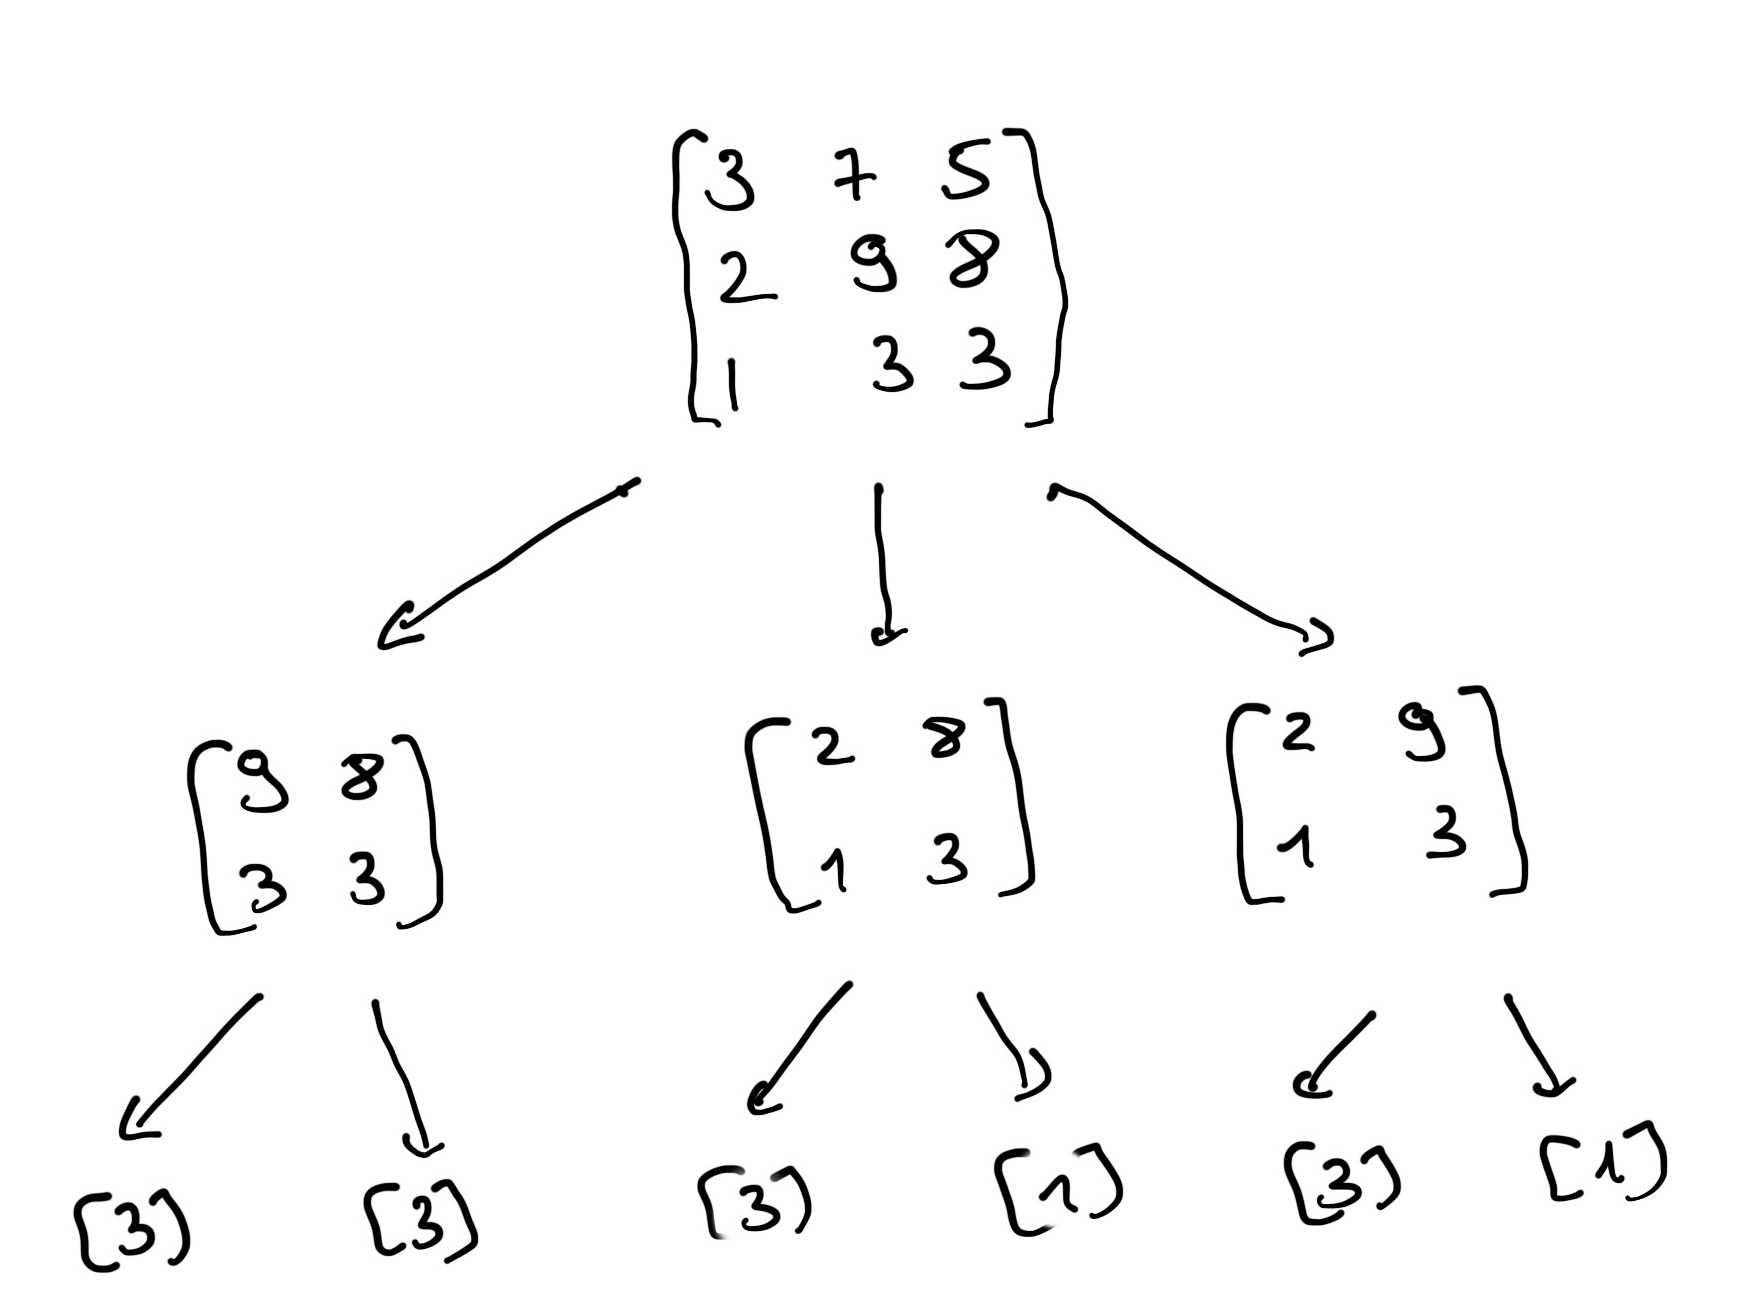
\includegraphics[height=5cm]{figures/DeterminantAlgoSlow.jpg}
  \caption{An example of the recursion tree of the algorithm from Example~\ref{exe:det}. The tree corresponds to the run of the algorithm on input $\protect\smat{         3 & 7 & 5 \\ 2&9&8 \\ 1 & 3 & 3  }.$
} 
\end{figure}


\section*{Exercises} 


\begin{enumerate}
\item Find the binary representation of $134$. 
\item Show that the binary representation with leading bit one of a positive natural number is
 unique. \label{alg:ex2}
\item Show that there are $n$-bit numbers $a,b ∈ ℕ$ such that the  Euclidean algorithm on input $a$ and $b$ performs  $\Omega(n)$ arithmetic operations. \emph{Hint: Fibonacci numbers} 
\item Show $n! =  2^{\Omega({n \log n})}$. 
\item 
Let $A ∈ ℝ^{n ×n}$  and suppose that the $n^2$ components of $A$ are pairwise different.
Suppose that $B$ is a matrix that can be obtained from $A$ by deleting the first $k$ rows and some of the $k$ columns of $A$. How many (recursive) calls of the form $\det(B)$ does the algorithm of Example~\ref{exe:det} create? 
\item Let $A ∈ ℝ^{n ×n}$  and suppose that the $n^2$ components of $A$ are pairwise different. How many different submatrices can be obtained from $A$ by deleting the first $k$ rows and some set of $k$ columns? Conclude that the algorithm  of Example~\ref{exe:det} remains exponential, even if it does not expand repeated subcalls. 
\item Complete the  algorithm below such  that it adds two natural numbers  in binary representation  $a_0,\dots,a_{l-1}$,  $b_0,\dots,b_{l-1}$. What is the asymptotic running time (number of basic operations) of your algorithm? Can there be an asymptotically  faster algorithm? 

  \begin{tabbing}
    Input:~~ \= Two natural numbers $a$ and $b$  in their binary representation\\ 
    \>   $a_0,\dots,a_{l-1}$, $b_0,\dots,b_{l-1}$. \\
    Output: \> The binary representation $c_0,\dots,c_l$ of $a+b$ \\
\pushtabs 	
\\
   $\mathrm{carry} := 0$ \\
   {\bf for} \= $i=0, \dots, l-1$ \\
             \> $c_i = \mathrm{carry} + a_i + b_i \pmod{2} $\\
             \> $\mbox{carry} := $ \\
   $c_l := $  \\
   {\bf return} $c_0,\dots ,c_l$ \\   
\poptabs
  \end{tabbing} \label{item:ex:7}

\end{enumerate}

\section{Analysis of Gaussian elimination} 
\label{sec:analys-gauss-elim}

We recall Gaussian elimination. 

\begin{algorithm}[Gaussian elimination]
  \label{alg:3}
  \begin{tabbing}
    Input: $A ∈ ℚ^{m ×n}$  \\
    Output: \= $A'$ in row echelon form such that there exists an invertible \\ 
            \> $Q ∈ ℚ^{m × m}$ such that $Q⋅A = A'$ . \\
            \pushtabs 
\\
$A' := A$ \\
$i := 1$\\
{\bf while} \=  ($i≤m$)  \\
\> find \emph{minimal} $1 ≤ j ≤n$ such that there exists $k≥i$ such that $a'_{kj} ≠ 0$ \\
\> If no such element exists, then {\bf stop} \\
            \> swap rows $i$ and $k$ in $A'$ \\
            \>  {\bf for} \= $k = i+1,\dots, m$ \\
            \>            \> subtract $(a'_{kj}/a'_{ij})$ times row $i$ from row $k$ in $A'$  \\
\> $i:=i+1$ 
\poptabs        
  \end{tabbing}
\end{algorithm}

\noindent 
We can easily prove correctness of the algorithm. First of all, the algorithm does only perform elementary row-operations of the form 
\begin{enumerate}[i)]
\item swap two rows 
\item subtract a multiple of one row from \emph{another} row. 
\end{enumerate}
This means that the resulting matrix $A'$ can be obtained via 
\begin{displaymath}
  A' = Q ⋅ A
\end{displaymath}
with a non-singular $Q ∈ ℚ^{m × m}$. On the other hand we have the following invariant. 
\begin{quote}
  After each iteration of the while-loop, the matrix $H$ obtained from the first  first $j$ columns of $A'$ is  in row-echelon form and rows $i,i+1,\dots,m$ of $H$  are entirely zero, see Figure\ref{fig:9}.  
\end{quote}

\begin{figure}  
   \centering
  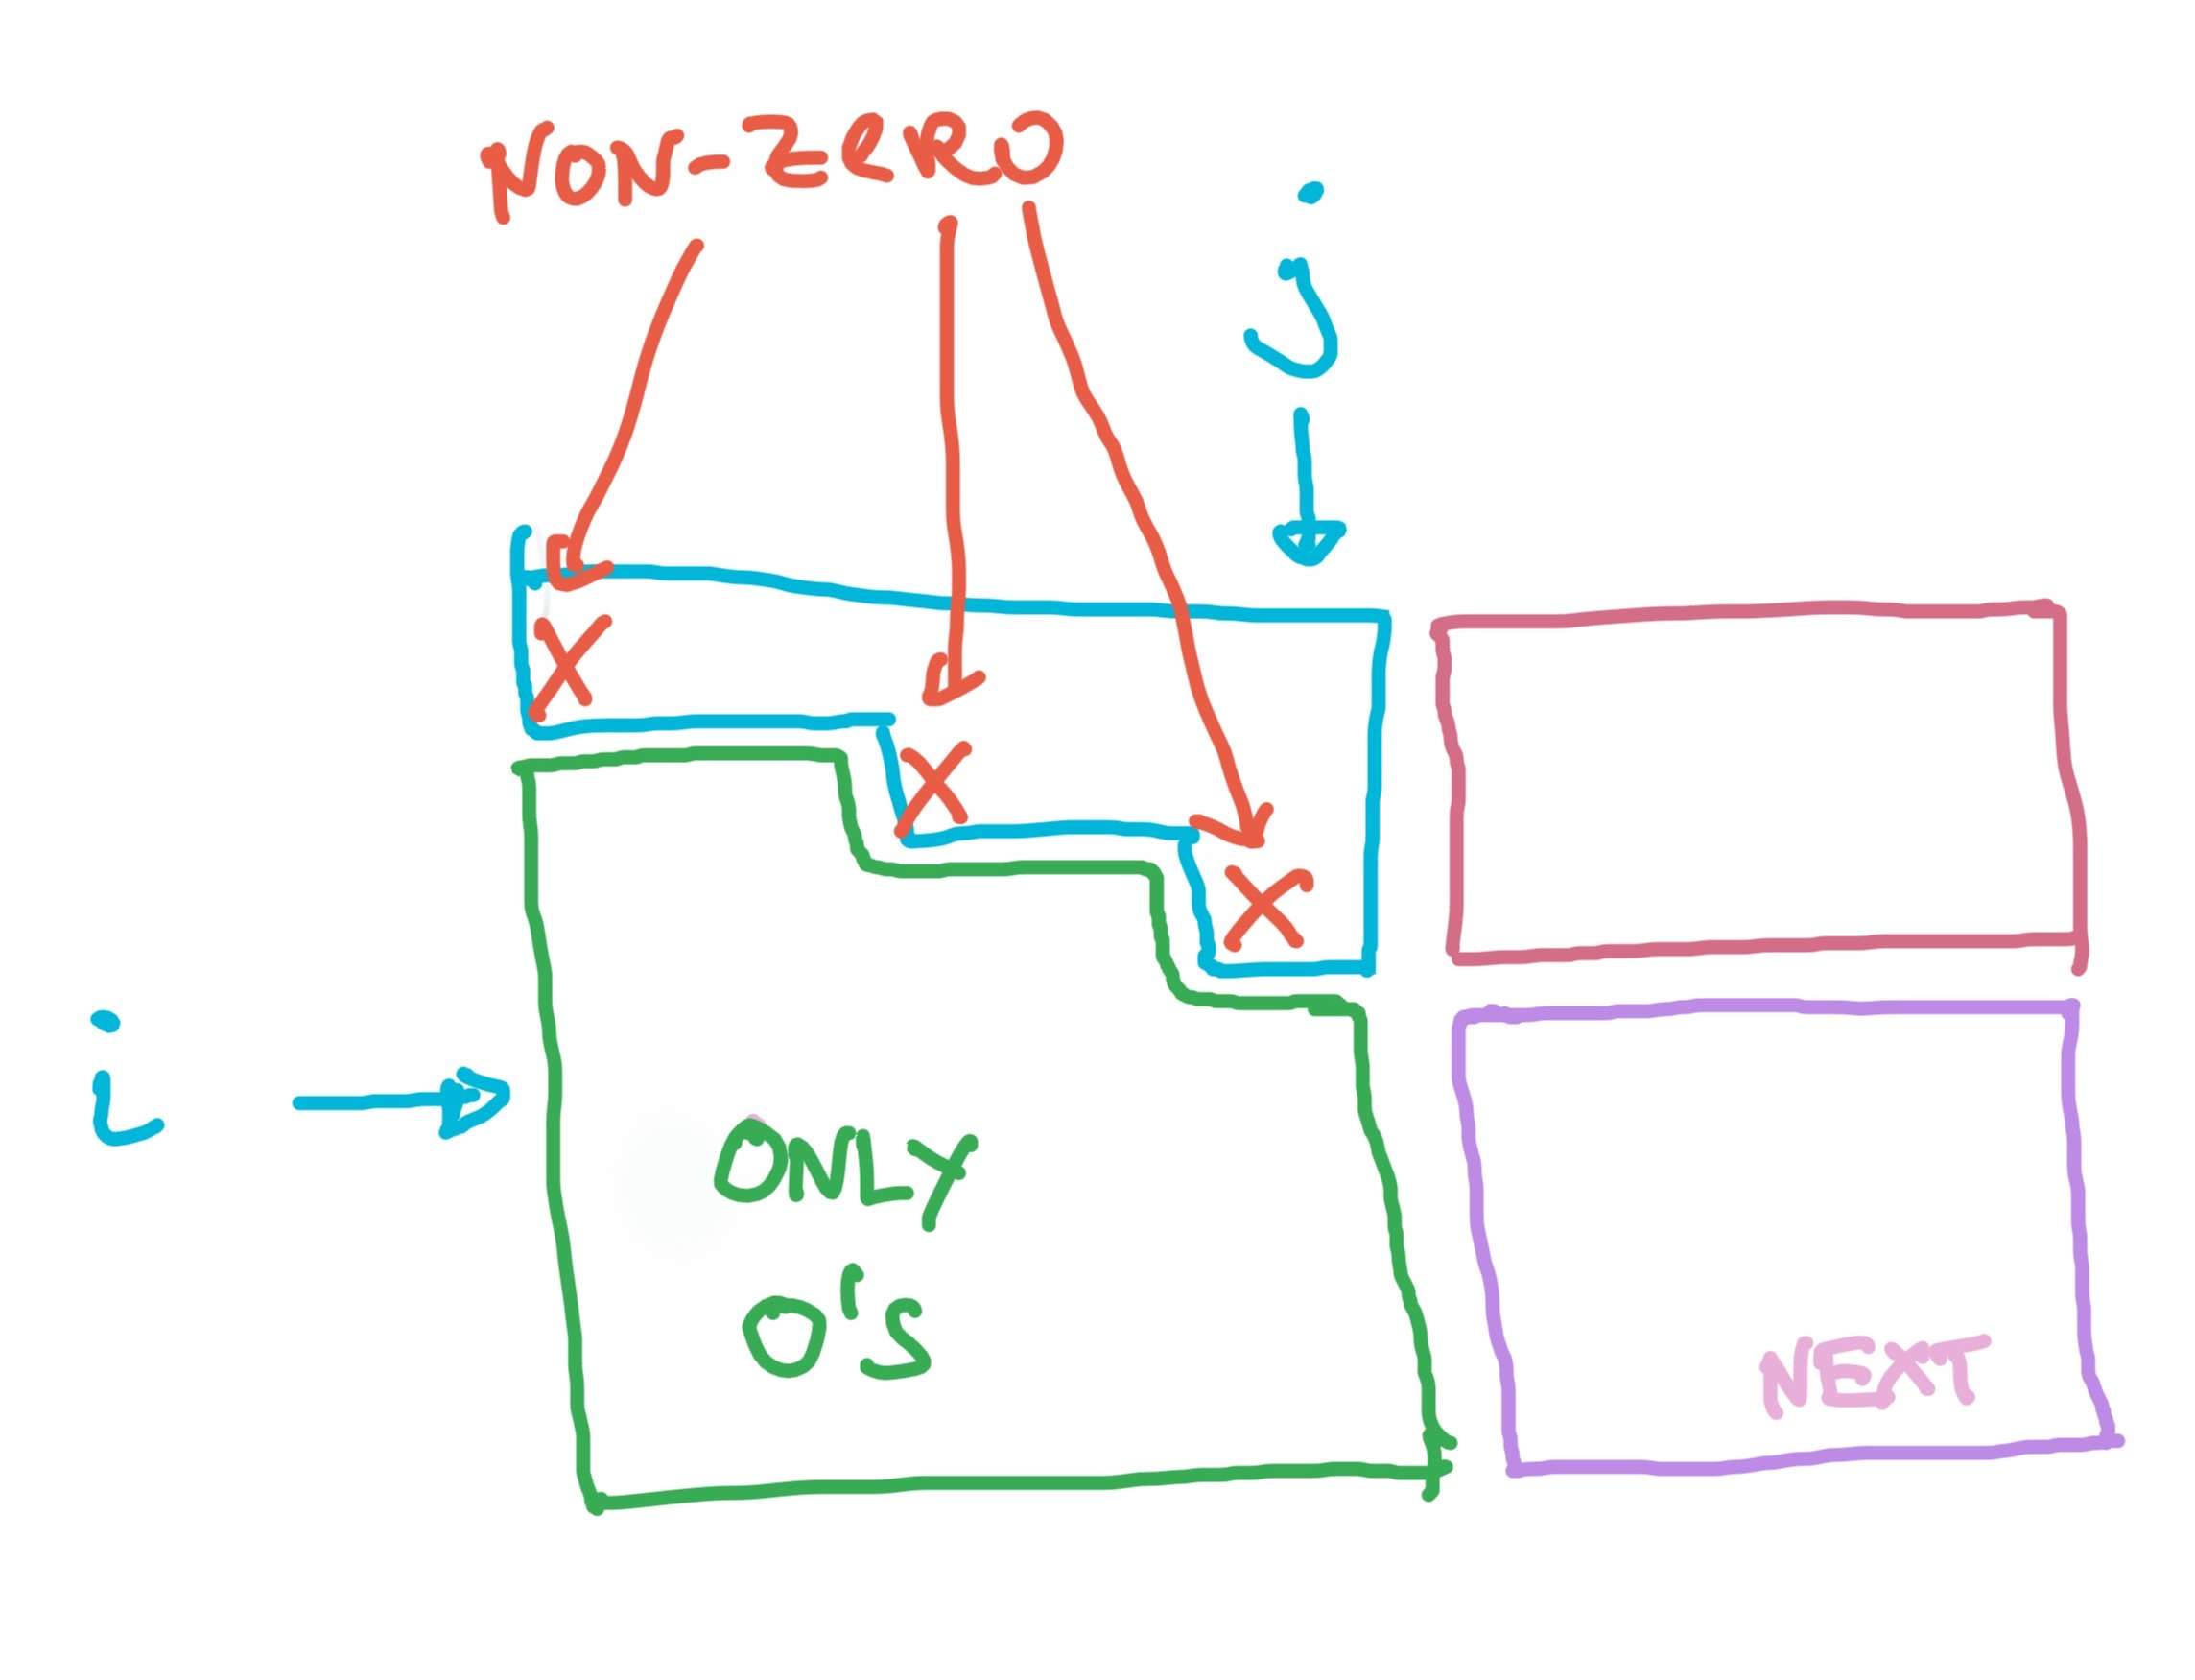
\includegraphics[height=5cm]{figures/Echelon.jpg}
  \caption{Gaussian elimination: The matrix $A'$ before  the $i$-th iteration of the while loop. \label{fig:9}}
\end{figure}


How many arithmetic operations does Gaussian elimination perform? Subtracting a multiple of one row from another row in $A'$ can be done in time $O(n)$ Thus the number of operations that are performed within the {\bf for}-loop are $O(m ⋅n)$ in total. There are $O(m)$ iterations through the while-loop. All-together this shows that Gaussian elimination performs $O(m^2 ⋅n)$ iterations. But how large can the numbers grow in the course of the Gaussian algorithm? Could it be that numbers have to be manipulated, whose binary encoding length is not polynomial in the total encoding length of the matrix $A$? Luckily the answer to this question is ``No''. To provide this answer, we have to show the following. 


\begin{theorem}[Hadamard bound] 
  Let $A \in \R^{n \times n}$ be non-singular. Then 
  \begin{displaymath}
    |\det(A)| \leq \prod_{i=1}^n \|a_i\|_2 \leq n^{n/2} \cdot B^n, 
  \end{displaymath}
  where $B$ is upper bound on absolute values of entries of $A$.
\end{theorem}

\begin{proof}
  The Gram-Schmidt orthogonalization of $A$ yields a factorization 
  \begin{displaymath}
    A = Q \cdot R,
  \end{displaymath}
where $R$ is an upper triangular matrix with ones on the diagonal. The matrix $Q$ has orthogonal columns, where the length of the $i$-th column $q^{(i)}$ is upper bounded by the length of the $i$-th column of $A$. 
The assertion follows from 
\begin{displaymath}
  \det(A)^2 = \det(Q)^2 = \det(Q^T) \det(Q) = \prod_i \|q^{(i)}\|^2. 
\end{displaymath}
\end{proof}



\begin{corollary}
\label{co:11}
  If $A\in \setZ^{n\times n}$ is integral and each entry in absolute
  value is bounded by $B$, then $\size(\det(A)) = O(n \log n+ n \cdot
  \size(B))$.
\end{corollary}
% 


\begin{corollary}
  \label{co:10}
   If $A\in \setQ^{n\times n}$ is a rational matrix and $φ$ is an upper bound on the size of each component of $A$, then $\size(\det(A)) = O( n^3 \cdot
  φ)$.
\end{corollary}

\begin{proof}
Suppose that $a_{ij} = p_{ij}/q_{ij}$ for each $ij$, where $p$ and $q$ are integers with $gcd(p,q)=1$. Then $(∏_{ij}q_{ij}) A$ is an integer matrix  and 
\begin{displaymath}
  \det(A) = (∏_{ij}q_{ij})^n \det((∏_{ij}q_{ij}) A). 
\end{displaymath}
The size of $(∏_{ij}q_{ij})^n $ is $O(n^2 φ)$ and the size of $\det((∏_{ij}q_{ij}) A$ is $O(n^3 φ)$ with Corollary~\ref{co:11} . 
\end{proof}


Now that we have shown that the determinant of a rational matrix is a number of polynomial encoding length, we can prove that Gaussian elimination is indeed a polynomial time algorithm.

\begin{theorem}
  \label{thr:9}
The   Gaussian algorithm runs in polynomial time. 
\end{theorem}

 
\begin{proof}
  Consider the matrix $A'$
  just before the $i$-th
  iteration of the while loop.  We need to show that each entry of the
  part of $A'$
  that still has to be transformed (the magenta-colored part of the
  matrix in Figure~\ref{fig:9}) is of polynomial size in the input
  encoding.

  We assume that the row-swaps of $A$
  have been done in advance, so that no further swaps occur during the
  algorithm.  Consider the absolute value of the product of the pivot
  elements (red $x$'s
  in the Figure). This  is the absolute value of the
  determinant of the submatrix of $A$,
  that is obtained by choosing the first $i-1$
  rows and the columns in which the pivot elements lie.  By
  Corollary~\ref{co:10} this rational number is of polynomial size in
  the input encoding of this sub-matrix and thus of $A$.

 Now, consider a nonzero element $z$
 in the part of $A'$
 that still needs to be transformed (the magenta part in
 Figure~\ref{fig:9}). The absolute value of the product of this
 element with the pivot elements is the absolute value of the
 submatrix that is obtained by choosing the first $i-1$
 rows and the row in which $z$
 lies and the columns in which the pivot-elements and $z$
 lie.  Therefore, the rational number $z$
 itself  is of polynomial encoding length in the input.
\end{proof}






\section*{Exercises} 
\label{sec:exercises}

\begin{enumerate}
\item \label{item:3} Show that the matrix $Q ∈ ℚ^{m × m}$ that transforms $A \in ℚ^{m × n}$ into $A'$ in the Gaussian algorithm via $Q ⋅A = A'$ has entries that are od polynomial size in the binary encoding length of $A$. 
\end{enumerate}


\section{Fast matrix multiplication} 
\label{sec:fast-matr-mult}


We conclude this chapter on the analysis of algorithms with a result
of Volker Strassen~\cite{strassen1969gaussian} who showed that two
$n ×n$
matrices can be multiplied in time (number of arithmetic operations)
$O(n^{2.805})$.
This algorithm was published in 1969 and it showed as well that a
matrix can be inverted within the same timebound, see~\cite{AHU74}. 

Our task is to compute the product 

\begin{equation}
  \label{eq:str:1}
C =   A \cdot B  
\end{equation}
for two $n ×n$ matrices. We have seen that straightforward matrix-multiplication (Example~\ref{ex-a-1}) requires $O(n^3)$ arithmetic operations. 
We can assume, by padding $A$ and $B$ with zeroes, that $n = 2^\ell$ for some $\ell ∈ ℕ_0$. 

If we split the matrices $A$ and $B$ into 4 $n/2 × n/2$ matrices 
\begin{equation}
  \label{eq:str:3}
  A =
  \begin{pmatrix}
    A_{11} & A_{12} \\ 
    A_{21} & A_{22} 
  \end{pmatrix} \, \text{ and }  B =
  \begin{pmatrix}
    B_{11} & B_{12} \\ 
    B_{21} & B_{22} 
  \end{pmatrix}
\end{equation}
Then 
\begin{displaymath}
  \begin{pmatrix}
    C_{11} & C_{12} \\
    C_{21} & C_{22}
  \end{pmatrix}
   =
  \begin{pmatrix}
    A_{11}\cdot B_{11} + A_{12}\cdot B_{21} & \, &  A_{11}\cdot B_{12} + A_{12}\cdot B_{22}  \\
        A_{21}\cdot B_{11} + A_{22}\cdot B_{21} &\, &     A_{21}\cdot B_{12} + A_{22}\cdot B_{22} 
  \end{pmatrix}.
\end{displaymath}
Thus wan can reduce \emph{one}   multiplication of two $n ×n$ matrices to $8$ multiplications of two $n/2 × n/2$ matrices. For the running time, one obtains the recurrence 
\begin{equation}
  \label{eq:stra:4}
  T(n ) = 8 \cdot T(n/2) + Θ(n^2) 
\end{equation}
which leads again to $T(n) = Θ(n^3)$, see exercise \ref{item:str:4}). 

Strassen discovered that one can preprocess the input matrices in such a way that the correct result can be retrieved from the result  $7$ multiplications of $n/2 × n/2$ matrices. The preprocessing and retrival time is $O(n)$ which yields the recursion 
\begin{equation}
  \label{eq:str:5}
  T(n) = 7 \cdot T(n/2) + O(n^2). 
\end{equation}

The idea is to compute the $7$ matrices
\begin{eqnarray*}
  M_1 & = & (A_{11} + A_{22}) \cdot (B_{11}+ B_{22}) \\
  M_2 & = & (A_{21} + A_{22}) \cdot B_{11} \\
  M_3 & = & A_{11} \cdot (B_{12} - B_{22}) \\
  M_4 & = & A_{22} \cdot (B_{21} - B_{11}) \\
  M_5 & = & (A_{11} + A_{12})\cdot B_{22} \\
  M_6 & = & (A_{21}-A_{11}) \cdot (B_{11}+B_{12}) \\
  M_7 & = & (A_{12}-A_{22}) \cdot  (B_{21} + B_{22})\\. 
\end{eqnarray*}
This amounts to $O(n^2)$ arithmetic operations and $7$ multiplications of $n/2 × n/2$ matrices. From $M_1,\dots,M_7$ one can retrieve 
\begin{eqnarray*}
C_{11} & = & M_1 + M_4 - M_5 + M_7\\
C_{12} & = & M_3 + M_5 \\
C_{21} & = & M_2 + M_4\\
C_{22} & = & M_1 - M_2 + M_3 + M_6.  
\end{eqnarray*}
again with $O(n^2)$ arithmetic operations. 


\begin{algorithm}[Fast matrix multiplication ($\mathrm{FMM}$)]

  \begin{tabbing}
    Input: Two $n ×n$ matrices $A$ and $B$ \\
    Output: $C = \mathrm{FMM}(A,B)$, the product $ A\cdot B$ \\

    {\bf if}  $n=1$ return $a_{11} ⋅b_{11}$ \\
    {\bf else} \=  \\
               \>  $M_1 = \mathrm{FMM} (A_{11} + A_{22} , B_{11}+ B_{22}) $ \\
               \> $M_2 = \mathrm{FMM}(A_{21} + A_{22},  B_{11})$ \\
               \> $M_3  = \mathrm{FMM} A_{11} , B_{12} - B_{22}) $\\
               \> $M_4  = \mathrm{FMM}( A_{22} , (B_{21} - B_{22})$ \\
               \> $M_5  = \mathrm{FMM}(A_{11} + A_{12}, B_{22})$ \\
               \> $M_6  = \mathrm{FMM} (A_{21}-A_{11}, B_{11}+B_{12}) $\\
               \> $M_7  = \mathrm{FMM} (A_{12}-A_{22}, B_{21} + B_{22})$\\ 
               \> Compute the matrices $C_{11}, C_{12}, C_{21}, C_{22}$ from $M_1,\dots,M_7$ \\
               \> {\bf return} $C$
  \end{tabbing}
\end{algorithm}

  \begin{figure}
    \centering
     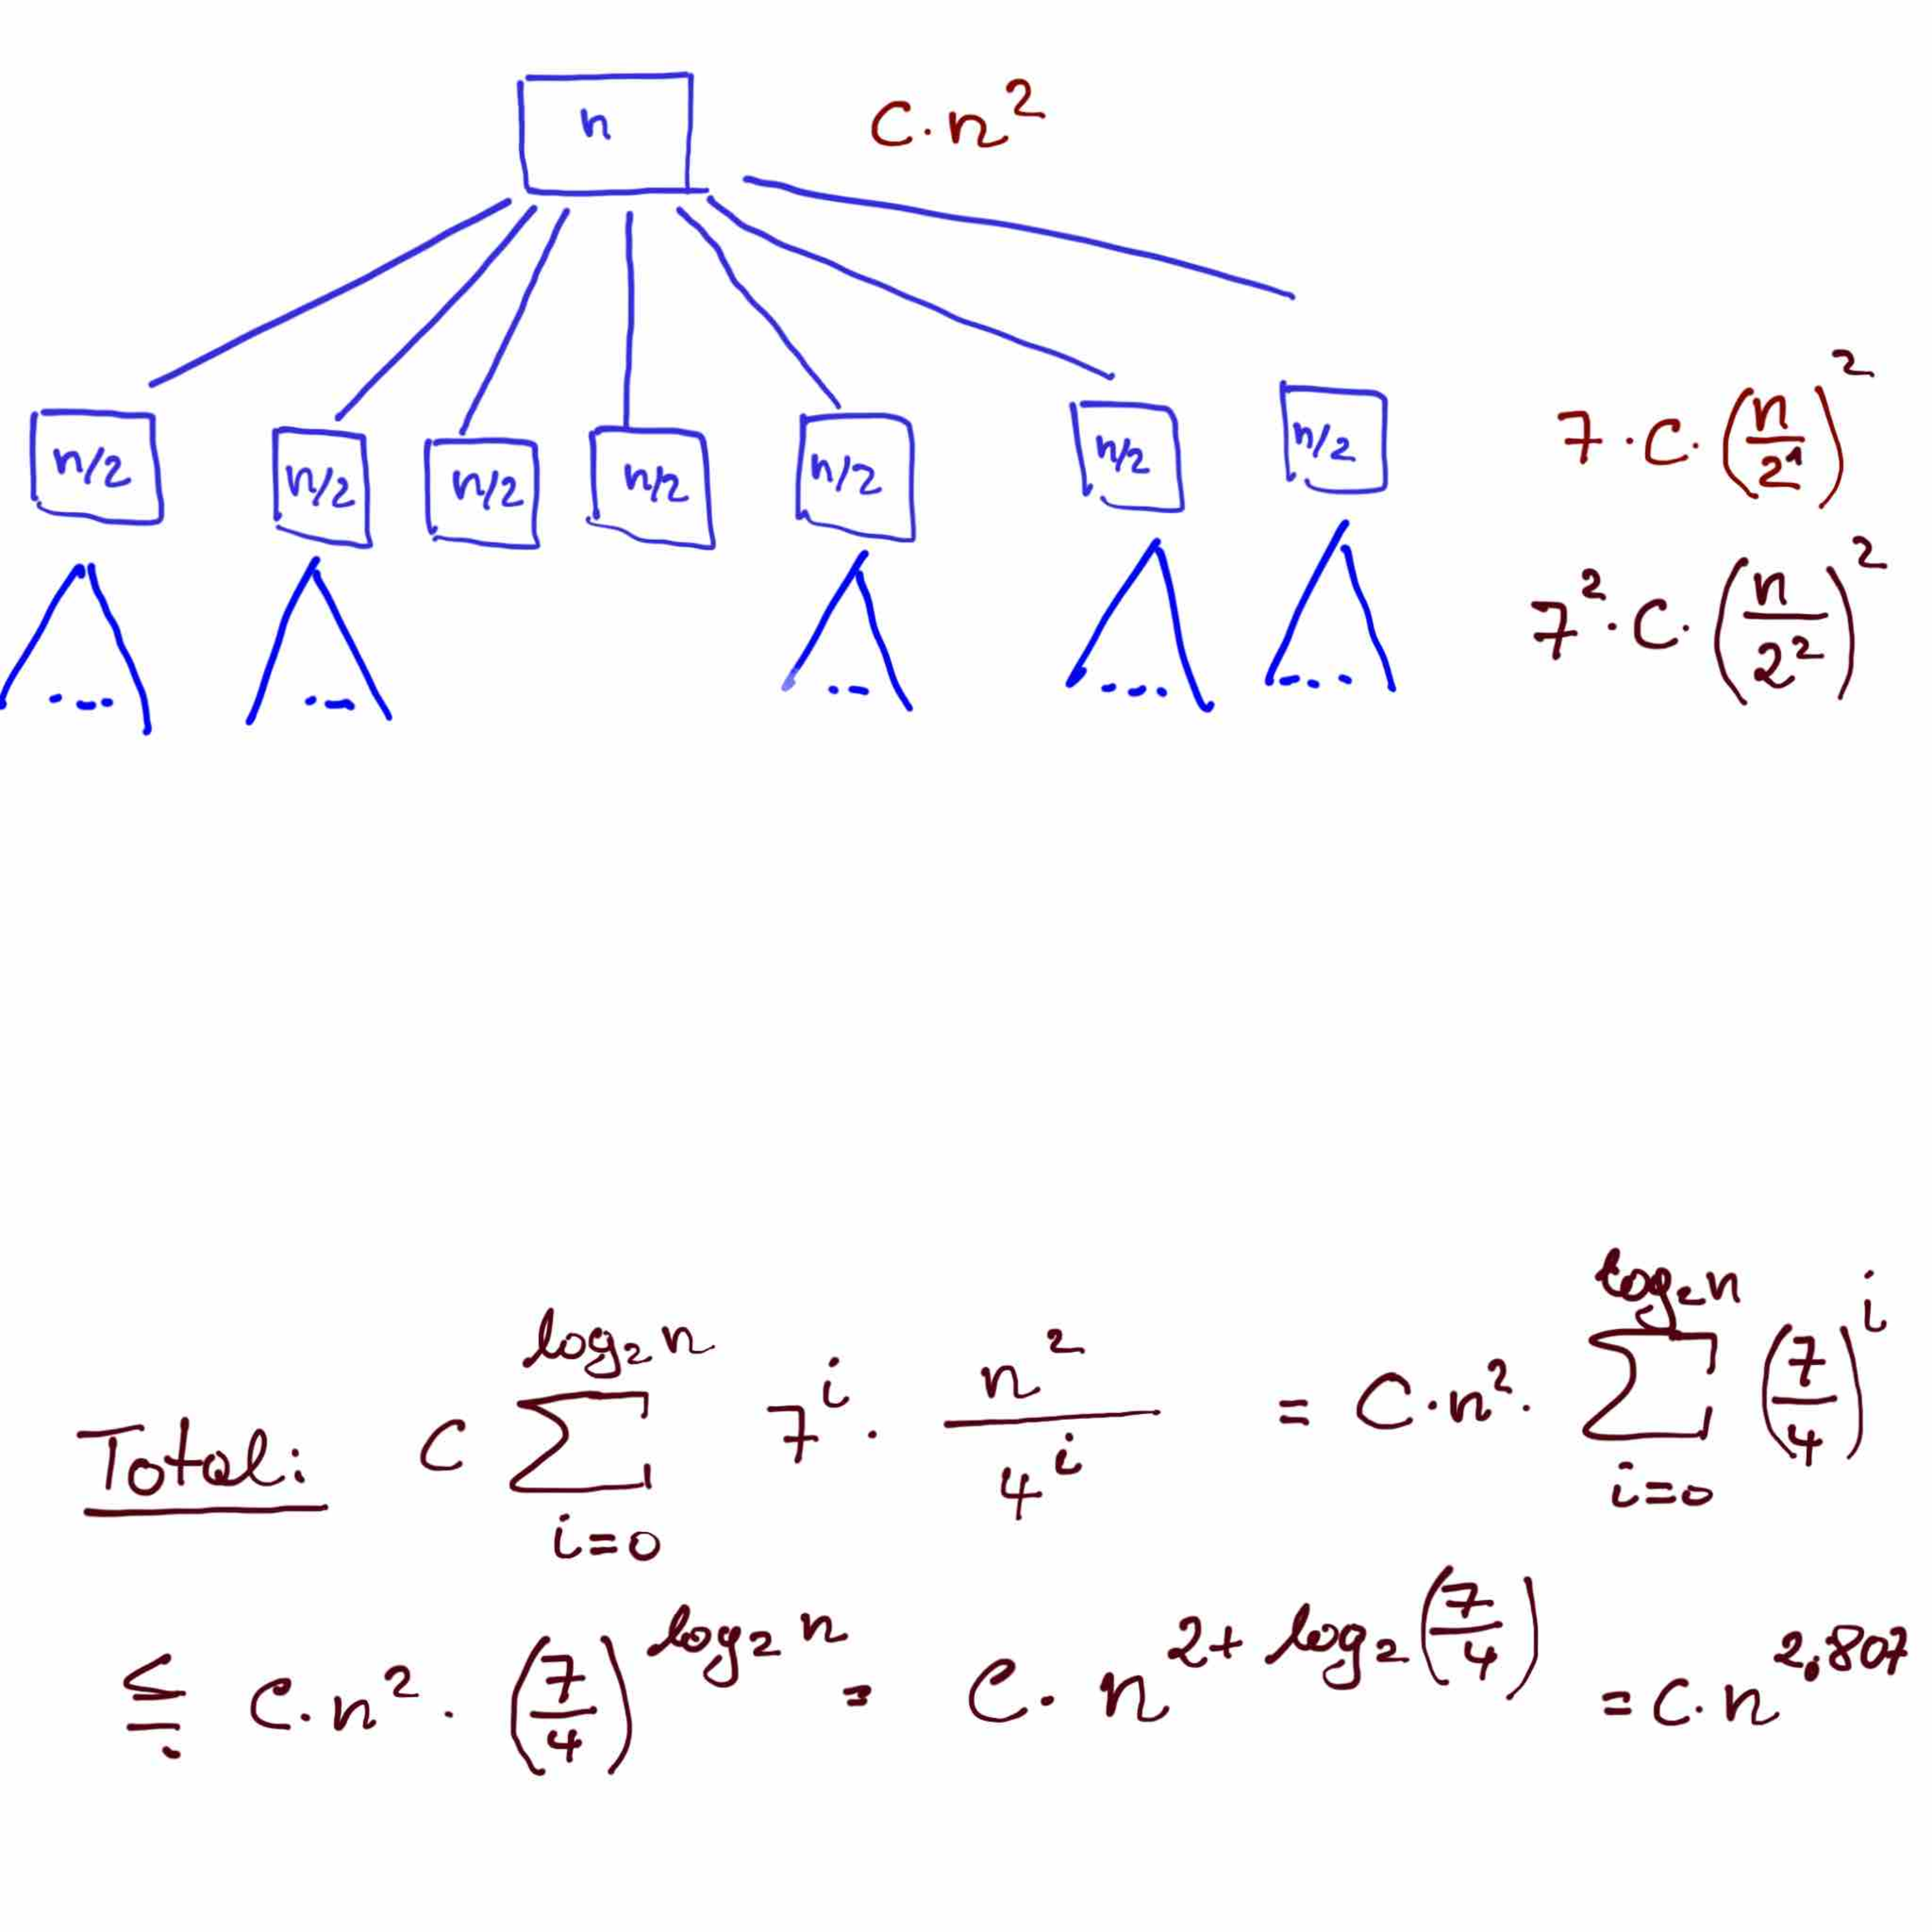
\includegraphics[height=8cm]{figures/Strassen2.pdf} 
    \caption{The analysis of the Strassen algorithm. }
    \label{fig:str:1}
  \end{figure}


  \begin{theorem}[Strassen]
    \label{thr:10}
    Two $n × n$ matrices can be multiplied in time (number of arithmetic operations) $O(n^{2+ \log_2(7/4)})$. 
  \end{theorem}



  \begin{proof}
    See Figure~\ref{fig:str:1}. 

  \end{proof}

\section*{Exercises}

\begin{enumerate}
\item Suppose we are given three $n×n$ matrices $A,B,C ∈ ℤ^{n×n}$ and we want to test whether $A ⋅ B = C$ holds. We could multiply $A$ and $B$ and then compare the result with $C$. This would amount to running time (number of arithmetic operations) of $O(n^3)$ with the standard matrix-multiplication algorithm. 

We now show how to perform an efficient \emph{randomized test}. Suppose that you can draw a vector $v ∈ \{0,1\}^n$  i.i.d. at random in time $O(n)$. The idea is then to compute the product $B ⋅v$ and then the product $A ⋅ (B ⋅v)$ and afterwards $C ⋅ v$, all in time $O(n^2)$. Show the following. 

\begin{enumerate}
\item If $A⋅B \neq C$, then $P(A ⋅ (B ⋅v) = C⋅v) ≤1/2$. 
\item Let $v_1,\dots,v_k∈ \{0,1\}^n$ be i.i.d. at random and suppose that  $A⋅B \neq C$. The probability of the event: $A ⋅ (B ⋅v_i) = C⋅v_i$ for each $i=1,\dots,k$ is bounded by $1/2^k$. 
\item Conclude that there is an algorithm that runs in time $O(k⋅n^2)$ which tests whether $A⋅B = C$ holds. The probability that the algorithm gives the wrong result is bounded by $1/2^k$. 
\end{enumerate}
\item Show that the recursion \eqref{eq:stra:4} has the solution $T(n) = Θ (n^3)$.  \label{item:str:4}
\item Describe an algorithm that multiplies two $n$-bit integers in time $O(n^2)$. You may use the algorithm to add two $n$-bit integers from exercise~\ref{cha:runn-time-analys}.\ref{item:ex:7}.  
\item Suppose $n = 2^\ell $  and $a,b ∈ ℕ$ are two $n$-bit integers. Consider the numbers $a_h$ and $a_l$ which are represented by the first $n/2$ bits and the last $n/2$ bits of $a$ respectively. Likewise the numbers $b_h$ and $b_l$ are the numbers represented by the first half and the second half of the bit-representation of $b$. 
  \begin{enumerate}[i)]
  \item Show $a = a_h ⋅ 2^{n/2} + a_l$ and  $b = b_h ⋅ 2^{n/2} + b_l$
  \item Show $a⋅b = a_h ⋅ b_h ⋅ 2^n + (a_h ⋅ b_l + a_l ⋅ b_h) ⋅2^{n/2} + a_l ⋅b_l$ 
  \item Conclude very carefully that two $n$-bit
    numbers can be multiplied by resorting to three multiplications of
    $n/2$-bit numbers and $O(n)$ basic  operations.
  \item Conclude that two $n$-bit
    numbers can be computed in time $O(n^{\log_2(3)})$
    elementary bit operations.
  \end{enumerate}




\end{enumerate}

%%% Local Variables:
%%% mode: latex
%%% TeX-master: "lecture"
%%% End:
